\documentclass{extbook}[14pt]
\usepackage{multicol, enumerate, enumitem, hyperref, color, soul, setspace, parskip, fancyhdr, amssymb, amsthm, amsmath, latexsym, units, mathtools}
\everymath{\displaystyle}
\usepackage[headsep=0.5cm,headheight=0cm, left=1 in,right= 1 in,top= 1 in,bottom= 1 in]{geometry}
\usepackage{dashrule}  % Package to use the command below to create lines between items
\newcommand{\litem}[1]{\item #1

\rule{\textwidth}{0.4pt}}
\pagestyle{fancy}
\lhead{}
\chead{Answer Key for Progress Quiz 4 Version A}
\rhead{}
\lfoot{5346-5907}
\cfoot{}
\rfoot{Summer C 2021}
\begin{document}
\textbf{This key should allow you to understand why you choose the option you did (beyond just getting a question right or wrong). \href{https://xronos.clas.ufl.edu/mac1105spring2020/courseDescriptionAndMisc/Exams/LearningFromResults}{More instructions on how to use this key can be found here}.}

\textbf{If you have a suggestion to make the keys better, \href{https://forms.gle/CZkbZmPbC9XALEE88}{please fill out the short survey here}.}

\textit{Note: This key is auto-generated and may contain issues and/or errors. The keys are reviewed after each exam to ensure grading is done accurately. If there are issues (like duplicate options), they are noted in the offline gradebook. The keys are a work-in-progress to give students as many resources to improve as possible.}

\rule{\textwidth}{0.4pt}

\begin{enumerate}\litem{
Choose the graph of the equation below.
\[ f(x) = \frac{1}{(x - 1)^2} + 1 \]The solution is the graph below, which is option E.
    \begin{center}
        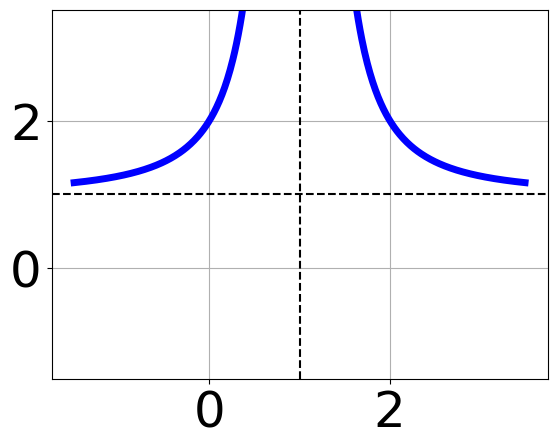
\includegraphics[width=0.3\textwidth]{../Figures/rationalEquationToGraphEA.png}
    \end{center}\begin{enumerate}[label=\Alph*.]
\begin{multicols}{2}
\item 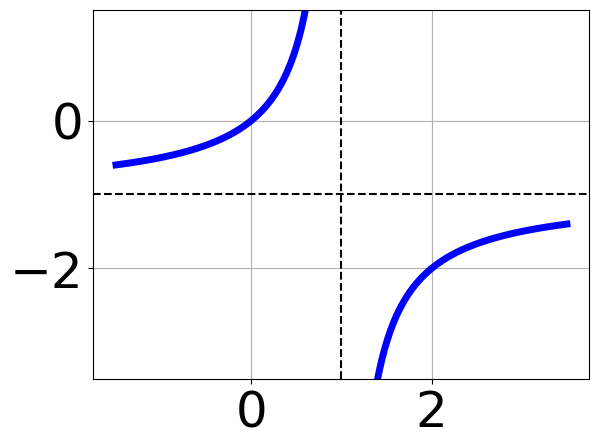
\includegraphics[width = 0.3\textwidth]{../Figures/rationalEquationToGraphAA.png}
\item 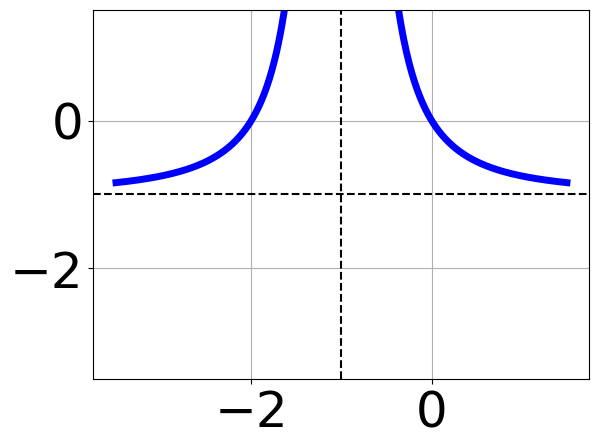
\includegraphics[width = 0.3\textwidth]{../Figures/rationalEquationToGraphBA.png}
\item 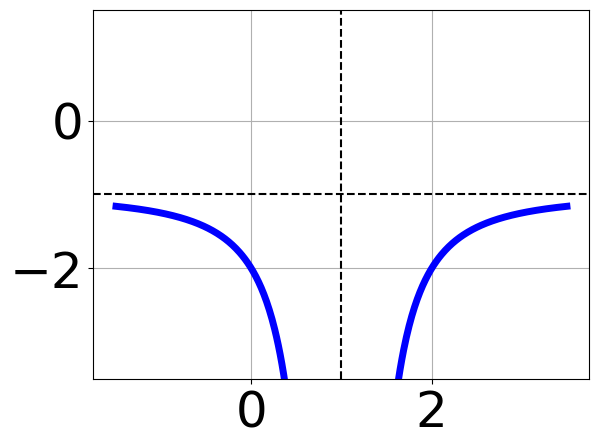
\includegraphics[width = 0.3\textwidth]{../Figures/rationalEquationToGraphCA.png}
\item 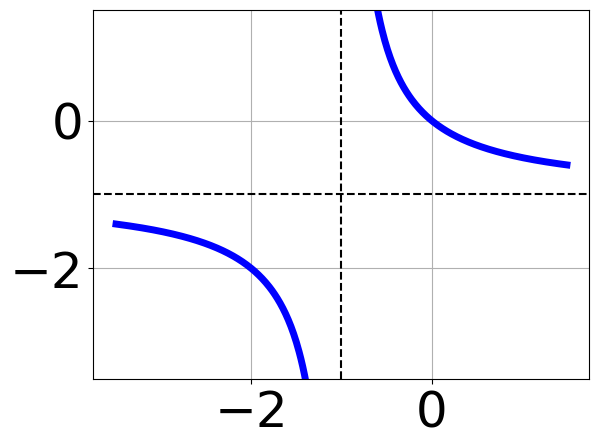
\includegraphics[width = 0.3\textwidth]{../Figures/rationalEquationToGraphDA.png}
\end{multicols}\item None of the above.\end{enumerate}
\textbf{General Comment:} Remember that the general form of a basic rational equation is $ f(x) = \frac{a}{(x-h)^n} + k$, where $a$ is the leading coefficient (and in this case, we assume is either $1$ or $-1$), $n$ is the degree (in this case, either $1$ or $2$), and $(h, k)$ is the intersection of the asymptotes.
}
\litem{
Choose the equation of the function graphed below.

\begin{center}
    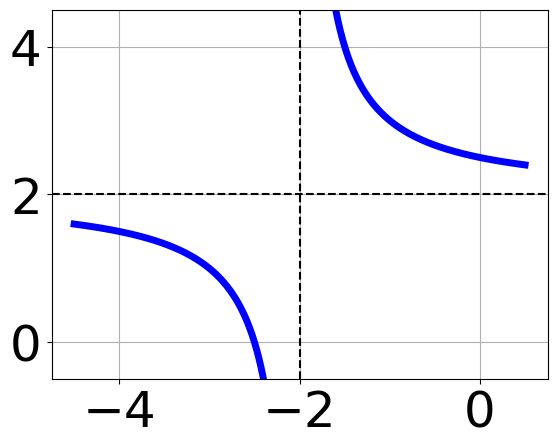
\includegraphics[width=0.5\textwidth]{../Figures/rationalGraphToEquationCopyA.png}
\end{center}


The solution is \( \text{None of the above as it should be } f(x) = \frac{1}{x + 2} + 2 \), which is option E.\begin{enumerate}[label=\Alph*.]
\item \( f(x) = \frac{-1}{(x + 2)^2} + 2 \)

Corresponds to thinking the graph was a shifted version of $\frac{1}{x^2}$, using the general form $f(x) = \frac{a}{x-h}+k$, and the opposite leading coefficient.
\item \( f(x) = \frac{-1}{x + 2} + 2 \)

Corresponds to using the general form $f(x) = \frac{a}{x-h}+k$ and the opposite leading coefficient.
\item \( f(x) = \frac{1}{x - 2} + 2 \)

The $x$-value of the equation does not match the graph.
\item \( f(x) = \frac{1}{(x - 2)^2} + 2 \)

Corresponds to thinking the graph was a shifted version of $\frac{1}{x^2}$.
\item \( \text{None of the above} \)

None of the equation options were the correct equation.
\end{enumerate}

\textbf{General Comment:} Remember that the general form of a basic rational equation is $ f(x) = \frac{a}{(x-h)^n} + k$, where $a$ is the leading coefficient (and in this case, we assume is either $1$ or $-1$), $n$ is the degree (in this case, either $1$ or $2$), and $(h, k)$ is the intersection of the asymptotes.
}
\litem{
Choose the equation of the function graphed below.

\begin{center}
    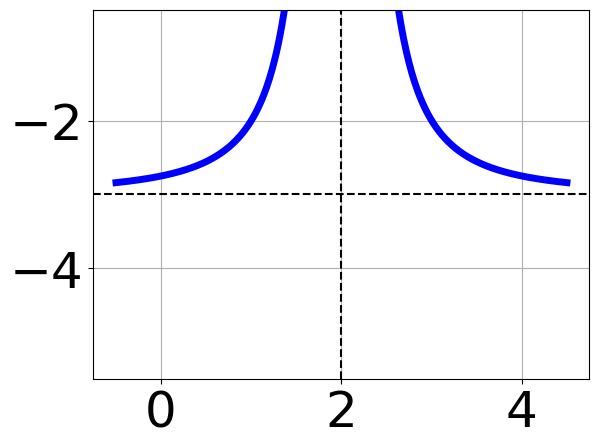
\includegraphics[width=0.5\textwidth]{../Figures/rationalGraphToEquationA.png}
\end{center}


The solution is \( \text{None of the above as it should be } f(x) = \frac{1}{(x - 2)^2} - 3 \), which is option E.\begin{enumerate}[label=\Alph*.]
\item \( f(x) = \frac{1}{(x + 2)^2} + 4 \)

The $x$- and $y$-value of the equation does not match the graph.
\item \( f(x) = \frac{-1}{(x - 2)^2} + 4 \)

Corresponds to using the general form $f(x) = \frac{a}{(x-h)^2}+k$, the opposite leading coefficient, AND not noticing the $y$-value was wrong.
\item \( f(x) = \frac{-1}{x - 2} + 4 \)

Corresponds to thinking the graph was a shifted version of $\frac{1}{x}$, using the general form $f(x) = \frac{a}{(x-h)^2}+k$, the opposite leading coefficient, AND not noticing the $y$-value was wrong.
\item \( f(x) = \frac{1}{x + 2} + 4 \)

Corresponds to thinking the graph was a shifted version of $\frac{1}{x}$ AND not noticing the $y$-value was wrong.
\item \( \text{None of the above} \)

None of the equation options were the correct equation.
\end{enumerate}

\textbf{General Comment:} Remember that the general form of a basic rational equation is $ f(x) = \frac{a}{(x-h)^n} + k$, where $a$ is the leading coefficient (and in this case, we assume is either $1$ or $-1$), $n$ is the degree (in this case, either $1$ or $2$), and $(h, k)$ is the intersection of the asymptotes.
}
\litem{
Solve the rational equation below. Then, choose the interval(s) that the solution(s) belongs to.
\[ \frac{5}{9x -4} + -8 = \frac{-6}{-63x + 28} \]The solution is \( x = 0.502 \), which is option E.\begin{enumerate}[label=\Alph*.]
\item \( x_1 \in [-0.2, 2.1] \text{ and } x_2 \in [0.51,0.61] \)

$x = 0.502 \text{ and } x = 0.597$, which corresponds to getting the correct solution and believing there should be a second solution to the equation.
\item \( x_1 \in [-0.5, -0.2] \text{ and } x_2 \in [0.43,0.53] \)

$x = -0.387 \text{ and } x = 0.502$, which corresponds to getting the correct solution and believing there should be a second solution to the equation.
\item \( x \in [-0.5,-0.2] \)

$x = -0.387$, which corresponds to not distributing the factor $9x -4$ correctly when trying to eliminate the fraction.
\item \( \text{All solutions lead to invalid or complex values in the equation.} \)

This corresponds to thinking $x = 0.502$ leads to dividing by zero in the original equation, which it does not.
\item \( x \in [-0.5,1.5] \)

* $x = 0.502$, which is the correct option.
\end{enumerate}

\textbf{General Comment:} Distractors are different based on the number of solutions. Remember that after solving, we need to make sure our solution does not make the original equation divide by zero!
}
\litem{
Solve the rational equation below. Then, choose the interval(s) that the solution(s) belongs to.
\[ \frac{7x}{4x -3} + \frac{-3x^{2}}{-12x^{2} -19 x + 21} = \frac{-6}{-3x -7} \]The solution is \( \text{All solutions are invalid or lead to complex values in the equation.} \), which is option A.\begin{enumerate}[label=\Alph*.]
\item \( \text{All solutions lead to invalid or complex values in the equation.} \)

* The equation leads to solving $-18x^{2} -25 x -18=0$, which leads to complex solutions. This is the correct option.
\item \( x_1 \in [-0.32, 0.21] \text{ and } x_2 \in [-1.51,-0.74] \)

$x = 0.025 \text{ and } x = -1.414$, which corresponds to making the discriminant from the Quadratic Formula positive to avoid complex solutions.
\item \( x \in [-3.39,-1.55] \)

$x = -2.333$, which corresponds to solving $-3x -7 = 0$ and treating it as a solution to the equation.
\item \( x \in [0.73,1.4] \)

$x = 0.750$, which corresponds to solving $4x -3 = 0$ and treating it as a solution to the equation.
\item \( x_1 \in [0.73, 1.4] \text{ and } x_2 \in [-2.36,-2.22] \)

$x = 0.750 \text{ and } x = -2.333$, which corresponds to solving $4x -3 = 0$ and $-3x -7 = 0$ and treating them as solutions to the equation.
\end{enumerate}

\textbf{General Comment:} Distractors are different based on the number of solutions. Remember that after solving, we need to make sure our solution does not make the original equation divide by zero!
}
\litem{
Determine the domain of the function below.
\[ f(x) = \frac{5}{15x^{2} -37 x + 20} \]The solution is \( \text{All Real numbers except } x = 0.800 \text{ and } x = 1.667. \), which is option E.\begin{enumerate}[label=\Alph*.]
\item \( \text{All Real numbers except } x = a, \text{ where } a \in [0.67, 1.06] \)

All Real numbers except $x = 0.800$, which corresponds to removing only 1 value from the denominator.
\item \( \text{All Real numbers.} \)

This corresponds to thinking the denominator has complex roots or that rational functions have a domain of all Real numbers.
\item \( \text{All Real numbers except } x = a, \text{ where } a \in [14.93, 15.63] \)

All Real numbers except $x = 15.000$, which corresponds to removing a distractor value from the denominator.
\item \( \text{All Real numbers except } x = a \text{ and } x = b, \text{ where } a \in [14.93, 15.63] \text{ and } b \in [19.8, 21.54] \)

All Real numbers except $x = 15.000$ and $x = 20.000$, which corresponds to not factoring the denominator correctly.
\item \( \text{All Real numbers except } x = a \text{ and } x = b, \text{ where } a \in [0.67, 1.06] \text{ and } b \in [0.92, 2.78] \)

All Real numbers except $x = 0.800$ and $x = 1.667$, which is the correct option.
\end{enumerate}

\textbf{General Comment:} Recall that dividing by zero is not a real number. Therefore the domain is all real numbers \textbf{except} those that make the denominator 0.
}
\litem{
Solve the rational equation below. Then, choose the interval(s) that the solution(s) belongs to.
\[ \frac{-8}{-2x -5} + -8 = \frac{6}{-14x -35} \]The solution is \( x = -1.946 \), which is option A.\begin{enumerate}[label=\Alph*.]
\item \( x \in [-1.95,-0.95] \)

* $x = -1.946$, which is the correct option.
\item \( x_1 \in [-1.95, 0.05] \text{ and } x_2 \in [3.05,4.05] \)

$x = -1.946 \text{ and } x = 3.054$, which corresponds to getting the correct solution and believing there should be a second solution to the equation.
\item \( \text{All solutions lead to invalid or complex values in the equation.} \)

This corresponds to thinking $x = -1.946$ leads to dividing by zero in the original equation, which it does not.
\item \( x \in [3.05,4.05] \)

$x = 3.054$, which corresponds to not distributing the factor $-2x -5$ correctly when trying to eliminate the fraction.
\item \( x_1 \in [-1.95, 0.05] \text{ and } x_2 \in [-2.62,-0.62] \)

$x = -1.946 \text{ and } x = -1.625$, which corresponds to getting the correct solution and believing there should be a second solution to the equation.
\end{enumerate}

\textbf{General Comment:} Distractors are different based on the number of solutions. Remember that after solving, we need to make sure our solution does not make the original equation divide by zero!
}
\litem{
Solve the rational equation below. Then, choose the interval(s) that the solution(s) belongs to.
\[ \frac{-6x}{3x + 4} + \frac{-4x^{2}}{12x^{2} +28 x + 16} = \frac{7}{4x + 4} \]The solution is \( \text{All solutions are invalid or lead to complex values in the equation.} \), which is option D.\begin{enumerate}[label=\Alph*.]
\item \( x_1 \in [-1.45, -1.13] \text{ and } x_2 \in [-1.26,0.58] \)

$x = -1.333 \text{ and } x = -1.000$, which corresponds to solving $3x + 4 = 0$ and $4x + 4 = 0$ and treating them as solutions to the equation.
\item \( x \in [-1.07,-0.84] \)

$x = -1.000$, which corresponds to solving $4x + 4 = 0$ and treating it as a solution to the equation.
\item \( x \in [-1.45,-1.13] \)

$x = -1.333$, which corresponds to solving $3x + 4 = 0$ and treating it as a solution to the equation.
\item \( \text{All solutions lead to invalid or complex values in the equation.} \)

* The equation leads to solving $-20x^{2} -45 x -28=0$, which leads to complex solutions. This is the correct option.
\item \( x_1 \in [-0.86, -0.73] \text{ and } x_2 \in [-2.56,-1.23] \)

$x = -0.758 \text{ and } x = -1.492$, which corresponds to making the discriminant from the Quadratic Formula positive to avoid complex solutions.
\end{enumerate}

\textbf{General Comment:} Distractors are different based on the number of solutions. Remember that after solving, we need to make sure our solution does not make the original equation divide by zero!
}
\litem{
Choose the graph of the equation below.
\[ f(x) = \frac{1}{x + 3} + 2 \]The solution is the graph below, which is option C.
    \begin{center}
        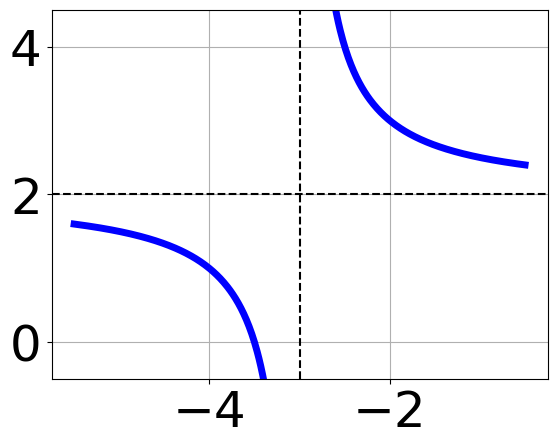
\includegraphics[width=0.3\textwidth]{../Figures/rationalEquationToGraphCopyCA.png}
    \end{center}\begin{enumerate}[label=\Alph*.]
\begin{multicols}{2}
\item 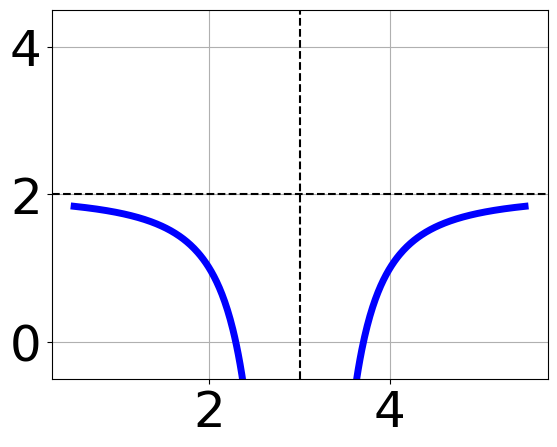
\includegraphics[width = 0.3\textwidth]{../Figures/rationalEquationToGraphCopyAA.png}
\item 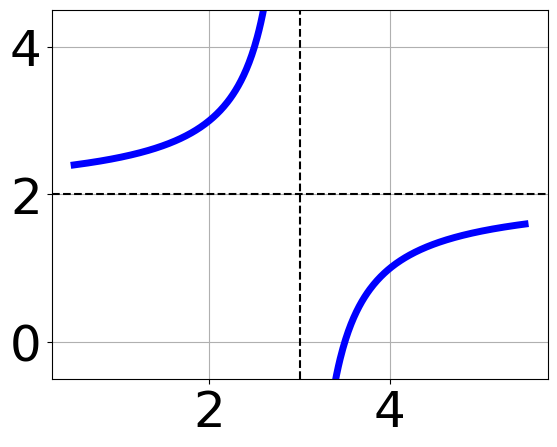
\includegraphics[width = 0.3\textwidth]{../Figures/rationalEquationToGraphCopyBA.png}
\item 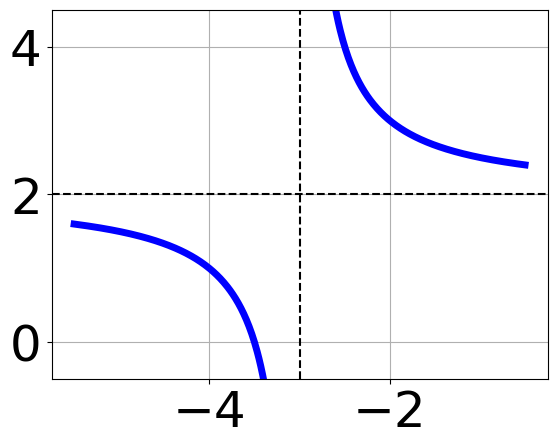
\includegraphics[width = 0.3\textwidth]{../Figures/rationalEquationToGraphCopyCA.png}
\item 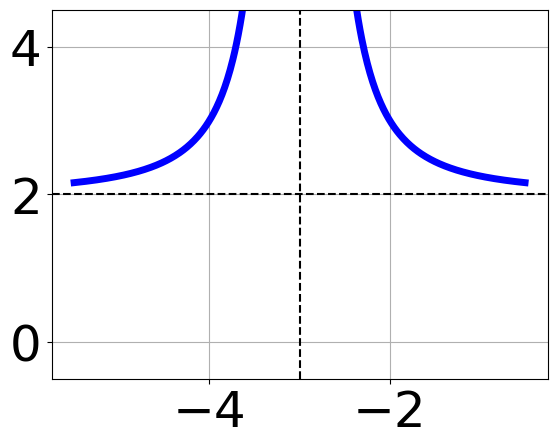
\includegraphics[width = 0.3\textwidth]{../Figures/rationalEquationToGraphCopyDA.png}
\end{multicols}\item None of the above.\end{enumerate}
\textbf{General Comment:} Remember that the general form of a basic rational equation is $ f(x) = \frac{a}{(x-h)^n} + k$, where $a$ is the leading coefficient (and in this case, we assume is either $1$ or $-1$), $n$ is the degree (in this case, either $1$ or $2$), and $(h, k)$ is the intersection of the asymptotes.
}
\litem{
Determine the domain of the function below.
\[ f(x) = \frac{4}{24x^{2} +34 x + 12} \]The solution is \( \text{All Real numbers except } x = -0.750 \text{ and } x = -0.667. \), which is option E.\begin{enumerate}[label=\Alph*.]
\item \( \text{All Real numbers except } x = a, \text{ where } a \in [-24.07, -23.74] \)

All Real numbers except $x = -24.000$, which corresponds to removing a distractor value from the denominator.
\item \( \text{All Real numbers except } x = a, \text{ where } a \in [-0.81, -0.75] \)

All Real numbers except $x = -0.750$, which corresponds to removing only 1 value from the denominator.
\item \( \text{All Real numbers except } x = a \text{ and } x = b, \text{ where } a \in [-24.07, -23.74] \text{ and } b \in [-12.04, -11.91] \)

All Real numbers except $x = -24.000$ and $x = -12.000$, which corresponds to not factoring the denominator correctly.
\item \( \text{All Real numbers.} \)

This corresponds to thinking the denominator has complex roots or that rational functions have a domain of all Real numbers.
\item \( \text{All Real numbers except } x = a \text{ and } x = b, \text{ where } a \in [-0.81, -0.75] \text{ and } b \in [-0.69, -0.66] \)

All Real numbers except $x = -0.750$ and $x = -0.667$, which is the correct option.
\end{enumerate}

\textbf{General Comment:} Recall that dividing by zero is not a real number. Therefore the domain is all real numbers \textbf{except} those that make the denominator 0.
}
\end{enumerate}

\end{document}